\section{Introducing HiQLab}

\subsection{\hiq\ description}

Electromechanical resonators and filters, such as quartz, ceramic, and
surface-acoustic wave devices, are important signal-processing
elements in communication systems.  Over the past decade, there has
been substantial progress in developing new types of miniaturized
electromechanical resonators using microfabrication processes.  For
these micro-resonators to be viable they must have high and
predictable quality factors ($Q$).  Depending on scale and geometry,
the energy losses that lower $Q$ may come from material damping,
thermoelastic damping, air damping, or radiation of elastic waves from
an anchor.  While commercial finite element codes can calculate the
resonant frequencies, they typically offer only limited support for
computing damping effects; and even if the software is capable of
forming the systems of equations that describe physically realistic
damping, there may not be algorithms to quickly solve those equations.

\hiq\ is a finite element program written to study damping in resonant
MEMS.  Though the program is designed with resonant MEMS in mind, the
architecture is general, and can handle other types of problems.  Most
architectural features in \hiq\ can be found in standard finite
element codes like FEAP; we also stole liberally from the code base
for the SUGAR MEMS simulator.

We wrote \hiq\ to be independent of any existing finite element code
for the following reasons:
\begin{itemize}

  \item We want to share our code, both with collaborators and with
  the community.  This is a much easier if the code does not depend on
  some expensive external package.

  \item We want to experiment with low-level details, which is more
  easily done if we have full access to the source code.

  \item We are mostly interested in linear problems, but they are
  problems with unusual structure.  It is possible to fit those
  structures into existing finite element codes, but if we have to
  write new elements, new solver algorithms, \emph{and} new assembly
  code in order to simulate anchor losses using perfectly matched
  layers, we get little added benefit to go with the cost and baggage
  of working inside a commercial code.

  \item We are still discovering which algorithms work well, and would
  like to be able to prototype our algorithms inside MATLAB.  We also
  want to be able to run multi-processor simulations outside of
  MATLAB, both to solve large problems and to run optimization loops.
  FEMLAB supports a MATLAB interface, but in our experience does not
  deal well with large simulations.  FEAP also supports a MATLAB
  interface (which we wrote), and the data structures in \hiq\ and
  FEAP are similar enough that we can share data between the two
  programs.

\end{itemize}

The main drawback of developing a new code is that we lack the pre-
and post-processing facilities of some other programs.


\subsection{\hiq\ architecture}

\begin{figure}
  \begin{center}
  \scalebox{1}{ \begin{picture}(0,0)
\ifx\pdfoutput\undefined
  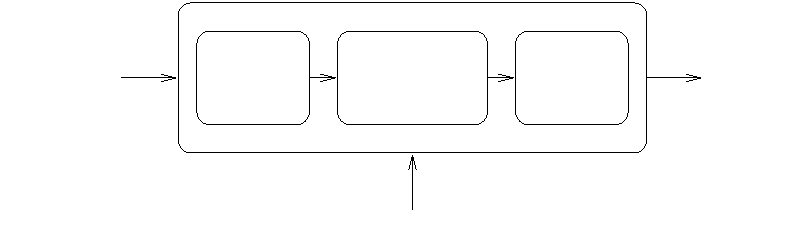
\includegraphics{hiq-arch.ps}
\else
  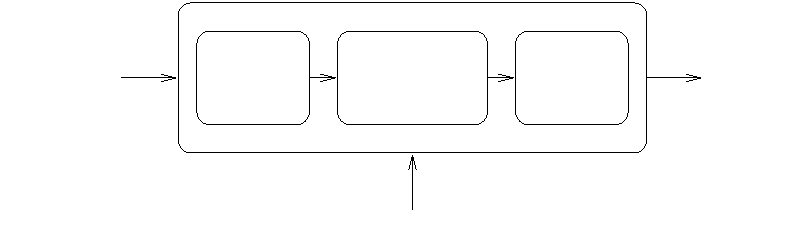
\includegraphics{hiq-arch.pdf}
\fi
\end{picture}
\setlength{\unitlength}{3947sp}%
%
\begingroup\makeatletter\ifx\SetFigFont\undefined%
\gdef\SetFigFont#1#2#3#4#5{%
  \reset@font\fontsize{#1}{#2pt}%
  \fontfamily{#3}\fontseries{#4}\fontshape{#5}%
  \selectfont}%
\fi\endgroup%
\begin{picture}(6374,1941)(376,-1315)
\put(6151,-61){\makebox(0,0)[lb]{\smash{{\SetFigFont{12}{14.4}{\familydefault}{\mddefault}{\updefault}{Results}%
}}}}
\put(376,-61){\makebox(0,0)[lb]{\smash{{\SetFigFont{12}{14.4}{\familydefault}{\mddefault}{\updefault}{Input deck}%
}}}}
\put(2701,-1261){\makebox(0,0)[lb]{\smash{{\SetFigFont{12}{14.4}{\familydefault}{\mddefault}{\updefault}{Programmatic user interface}%
}}}}
\put(2026,-61){\makebox(0,0)[lb]{\smash{{\SetFigFont{12}{14.4}{\familydefault}{\mddefault}{\updefault}{Models}%
}}}}
\put(3151,-61){\makebox(0,0)[lb]{\smash{{\SetFigFont{12}{14.4}{\familydefault}{\mddefault}{\updefault}{Assembly}%
}}}}
\put(4576,-61){\makebox(0,0)[lb]{\smash{{\SetFigFont{12}{14.4}{\familydefault}{\mddefault}{\updefault}{Solvers}%
}}}}
\end{picture}%
 }
  \end{center}
  \caption{Architecture of \hiq}
\end{figure}

The main components of \hiq\ are as follows.

\begin{itemize}
\item The mesh description language

The main way to describe devices in \hiq\ is to write a mesh input
deck using the Lua programming language (\ttt{http://www.lua.org}).
Because meshes are generated programmatically, it is easy to create
parameterized descriptions with hierarchies and arrays.

\item The programmatic user interfaces

There are two versions of the user interface: the MATLAB interface and
the standalone interface.  When using the MATLAB interface, a user has
access to the full range of MATLAB's numerical solvers and graphics
routines.  When using the standalone interface, a user does not have
as many built-in capabilities; but because the standalone interface
does not rely on MATLAB, it takes less memory and can solve larger
problems.  Like the mesh description interface, the user interface is
written in the Lua language, and is fully programmable.  We describe
both the MATLAB interface and the standalone interface in this manual.

\item The element model library

The element library includes linear, quadratic, and cubic quad and
brick elements for elastic problems and coupled thermoelastic problems
in plane strain, plane stress, axisymmetry, or three dimensions.  The
code also provides scalar wave equation elements in one, two, or three
dimensions.  For both scalar and elastic waves, the code supports
\emph{perfectly matched layer} sbsorbing boundaries to mimic the
effect of infinite domains.

\item The solver library

The solver library includes code for
\begin{itemize}
  \item Modal analysis of structures with anchor loss and
    thermoelastic damping.
  \item Forced response analysis, including forced response
    visualization and Bode plot construction.  The forced response
    analysis routines incorporate reduced order models.
\end{itemize}

\end{itemize}


\subsection{Download and basic setup}

The fastest way to get started with \hiq\ is to use the pre-compiled
version, available for Linux or Windows machines.  You can download
the source code and pre-compiled executables at
\begin{verbatim}
   http://www.cs.berkeley.edu/~dbindel/hiqlab/
\end{verbatim}
If you wish to run \hiq\ with the MATLAB interface, you will need
MATLAB version 6 or later.

If you wish to build your own version of \hiq, you will need
\begin{itemize}
  \item A C/C++ compiler and a FORTRAN 77 compiler (we have used the
    GNU compiler on Linux and Windows, and the Intel compilers on
    Itanium)
  \item Perl 5.002 or later
  \item LAPACK and BLAS (Basic Linear Algebra Subroutine) libraries.
    If you are compiling the MATLAB front-end for \hiq, these are
    already provided.
  \item UMFPACK (a linear system solver)
  \item ARPACK (an iterative eigenvalue solver)
\end{itemize}
If these packages are installed, you should be able to configure and
compile the software by running the following commands from the \hiq\
top-level directory:
\begin{verbatim}
  ./configure
  make
\end{verbatim}

At the time this manual is being written, \hiq\ is \emph{alpha}
software.  The code is still changing rapidly, and if you have trouble
setting up the program and running basic examples, please check to
make sure you have the most recent version.


\subsubsection{Running in MATLAB}

Once you have downloaded the pre-compiled version of the code (or once
you have built your own version), start MATLAB and run the file
\ttt{init.m}.  You should see something like the following:
\begin{verbatim}
 
                              < M A T L A B >
                  Copyright 1984-2001 The MathWorks, Inc.
                       Version 6.1.0.450 Release 12.1
                                May 18 2001
 
  
  To get started, type one of these: helpwin, helpdesk, or demo.
  For product information, visit www.mathworks.com.
  
>> init
HiQlab 0.2
Copyright   : Regents of the University of California
Build system: i686-pc-linux-gnu
Build date  : Tue Mar  1 12:51:22 PST 2005
Bug reports : dbindel@cs.berkeley.edu
>>
\end{verbatim}

\emph{You must run \ttt{init} before using \hiq from MATLAB.}  The
\ttt{init} script sets the MATLAB path variable so that MATLAB can
find the files \hiq\ needs for its analyses.

If you run \ttt{init} and see the \hiq\ banner, that means that you
have a working version of the MATLAB \hiq\ interface for your
machine.  If there is an error message when you run \ttt{init},
please send an e-mail including the exact error message, operating
system version, and MATLAB version.


\subsubsection{Running in standalone mode}

If you want to use the standalone version, look for an executable file
called \ttt{hiqlab} in the \ttt{src/lua} subdirectory.  When you
run \ttt{hiqlab} with no arguments, you should see an banner with
program information and a control prompt:
\begin{verbatim}
[dbindel@localhost lua]$ ./hiqlab
-------------------------------------------------------
HiQlab 0.2
Copyright   : Regents of the University of California
Build system: i686-pc-linux-gnu
Build date  : Thu Mar  3 19:29:03 PST 2005
Bug reports : dbindel@cs.berkeley.edu
 
Lua 5.0.2  Copyright (C) 1994-2004 Tecgraf, PUC-Rio
-------------------------------------------------------
 
>
\end{verbatim}%$
To end the \hiq\ session, press Ctrl-D on the keyboard.  \hiq\ may
also be run non-interactively: if \ttt{batch.lua} is a script that
runs an analysis and prints it out, for example, you might run
\begin{verbatim}
hiqlab batch.lua
\end{verbatim}

Like the MATLAB interface, the standalone user interface needs to know
where to find files.  The \ttt{init.lua} file in the \hiq\ main
directory specifies these files.  The first line of \ttt{init.lua}
has the form
\begin{verbatim}
HOME='/my/hiq/directory'
\end{verbatim}
where ``my hiq directory'' should be replaced by the directory
where \hiq\ is installed.  This is usually done automatically at
configuration time.  You can ensure that \hiq\ executes
\ttt{init.lua} when it starts in one of two ways:
\begin{enumerate}
\item Set the \ttt{HIQ\_INIT} environment variable to point to the
  full path for \ttt{init.lua}.  \hiq\ calls any files specified in
  the \hiq\ directory
\item Specify \ttt{init.lua} using the \ttt{-l} argument to
  \hiq.  For example, to execute \ttt{init.lua} before running
  \hiq\ in interactive mode,
\begin{verbatim}
hiqlab -l /my/hiq/directory/init.lua -i
\end{verbatim}
  and to run a batch script,
\begin{verbatim}
hiqlab -l /my/hiq/directory/init.lua batch.lua
\end{verbatim}
\end{enumerate}


\subsection{``Hello world'' in \hiq}

\subsubsection{Describing a cantilever beam}

\begin{figure}
\begin{verbatim}
require 'common.lua'
 
l = 10e-6         -- Beam length
w = 2e-6          -- Beam width
dense = 0.5e-6    -- Approximate element size (for block generator)
order = 2         -- Order of elements
 
mesh  = Mesh:new(2)
mat   = make_material('silicon2', 'planestrain')
mesh:blocks2d( { 0, l }, { -w/2.0, w/2.0 }, mat )
 
mesh:set_bc(function(x,y)
  if x == 0 then return 'uu', 0, 0; end
end)
\end{verbatim}
\caption{The complete mesh input file for a cantilever beam}
\label{mesh-input-fig}
\end{figure}

Figure~\ref{mesh-input-fig} shows the input file used to describe a
simple cantilever beam.  We now describe the input file in detail.  

\begin{itemize}

\item Including common support files:
\begin{verbatim}
require 'common.lua'
\end{verbatim}

Typically, input files will start with one or more \ttt{require}
statements, which are used to load function definitions, material
databases, and other data.  The \ttt{require} statement is much
like an include statement in C or Fortran, except that
\ttt{require} loads each file \emph{once}.  For example, the file
\ttt{common.lua} begins by requiring \ttt{material.lua}; if my
input file also started with a line \ttt{require 'material.lua'},
I would not end up with two copies of the material definitions file.

When the interpreter encounters a \ttt{require} statement, it
searches through a standard path to find a file with a matching name.
We will say more about the search path in
Section~\ref{require-section}.  The file \ttt{common.lua}, which is
defined in \ttt{models/common.lua} provides functions that are
useful for defining element types; \ttt{common.lua} should be
included in most mesh description files.

\item Defining geometric parameters:
\begin{verbatim}
l = 10e-6         -- Beam length
w = 2e-6          -- Beam width
\end{verbatim}

A two-dimensional beam model must have a length and a width.  These
two lines give the beam length (10 \mum) and width (2 \mum) in MKS
units.  Giving names to geometric parameters makes the input file
easier to read than it would otherwise be.  In
Section~\ref{parameterization-section}, we describe how named
parameters can be set from outside the input file in order to simplify
parameter studies.

\item Defining mesh generation parameters:
\begin{verbatim}
dense = 0.5e-6    -- Approximate element size (for block generator)
order = 2         -- Order of elements
\end{verbatim}

The mesh file must describe both the geometry of the device and the
parameters that define the mesh.  \hiq\ includes several functions
that define regular ``blocks'' that can be tied together to form a
mesh.  The \texttt{dense} and \texttt{order} parameters control how
\hiq\ builds these blocks.  The \texttt{order} parameter is the order
of polynomial interpolation used within each element: linear,
quadratic, and cubic elements are available.  The \texttt{dense}
parameter describes the element size.

\item Creating a mesh object:
\begin{verbatim}
mesh = Mesh:new(2)
\end{verbatim}

All information about the mesh is stored in a mesh object.  The mesh
constructor has a single argument, the dimension of the ambient space
for the problem.  The mesh object should be called \ttt{mesh}.

\item Defining a material:
\begin{verbatim}
mat = make_material('silicon2', 'planestrain')
\end{verbatim}

Build an element type for computing the response of silicon in plane
strain.  The first argument refers to an entry in \ttt{materials.lua}
which defines material arguments like Young's modulus and the Poission
ratio; subsequent arguments define the type of analysis (plane stress,
plane strain, axisymmetric, or three-dimensional).


\item Defining the mesh:
\begin{verbatim}
mesh:blocks2d( { 0, l }, { -w/2.0, w/2.0 }, mat )
\end{verbatim}

The mesh for a cantilever beam is simple: it covers the rectangular
region $[0,l] \times [-w/2,w/2]$.  The \ttt{blocks2d} generator
creates such a region and adds it to the mesh; the element size and
order are determined by the global variables \ttt{dense} and
\ttt{order} defined earlier, and the \ttt{mat} parameter from the
previous line defines which material should be used.


\item Defining boundary conditions:
\begin{verbatim}
mesh:set_bc(function(x,y)
  if x == 0 then return 'uu', 0, 0; end
end)
\end{verbatim}

By calling \ttt{mesh:set\_bc(myfunc)}, we define boundary conditions
for the problem.  \ttt{myfunc} may be an anonymous function (a
function without an explicitly assigned name), which is what we use
for this problem.  The function is called at every node in the mesh.
If the call returns nothing, then no boundary conditions are applied;
otherwise, the call returns a string which defines whether essential
or natural (displacement or flux) boundary conditions are applied.  In
this example, displacement boundary conditions (denoted by 'u') are
given for both the $x$ and $y$ displacements.  The two numeric
arguments after the string indicate that the $x$ and $y$ displacements
are set to zero.

\end{itemize}

\subsubsection{Eigenvalue analysis in MATLAB}
\subsubsection{Eigenvalue analysis in standalone mode}

\subsection{Getting help}
